\documentclass[12pt]{extarticle}

\setlength{\headheight}{16pt} % ??? we do what fancyhdr tells us to do  

\title{Mathematical Modelling for ML}
\author{Giacomo Ellero}
\date{a.y. 2024/2025}

\usepackage{preamble}

\renewcommand{\vec}[1]{\bvec{#1}}

\begin{document}

\oldfirstpage

\section{Introduction}

Assume our data is of the form $(x_n, y_n)$, where $x \in \R ^d$ and $y \in \R$
and we want to find a predictor $f_\theta(\cdot): \R^d \to \R$.

To figure out how good our model is we want to find a \emph{loss function} which tells us
how far is our predicted value from the real one.
Ideally we'd like to \say{count} the errors we make and use that as our loss function,
however these functions are usually not differentiable.
To fix this problem we look for another function which is differentiable and bounds the \say{true}
loss function, an example is the \emph{square error} (as we saw in statistics).
Eventually we want to find a model which minimizes the average loss:
\begin{equation}
	\argmin_\theta \bm R_\text{emp}(\theta) = \frac{1}{N} \sum_{i = 1}^N \ell(y_i, \hat y_i)
\end{equation}
Note that we will use $\theta$ and $w$ interchangeably,
they both represents the parameters/coefficients/weights of our model.

As we saw in linear regressions, the best estimator for $w$ is
\begin{equation}
	\hat w= (W^T W)^{-1} X^T y
\end{equation}
However, the Hessian matrix (given by $\laplacian \ell (w) = X^T X$)
is \emph{positive semi-definite}: this means that the function indeed has a global minimum,
but it might not be unique.
If we find more than one minimum we take the one which is closer to the origin:
in this way we avoid noise as much as possible.

\subsection{Reducing overfitting}
When we train our model we try to minimize the error against the training set.
Then we run the model against the test dataset:
of course we will get a higher loss than on the training set, however we want to check how the model
behaves when we modify the number of parameters to check for overfitting or underfitting.

\begin{figure}[H]
	\centering
	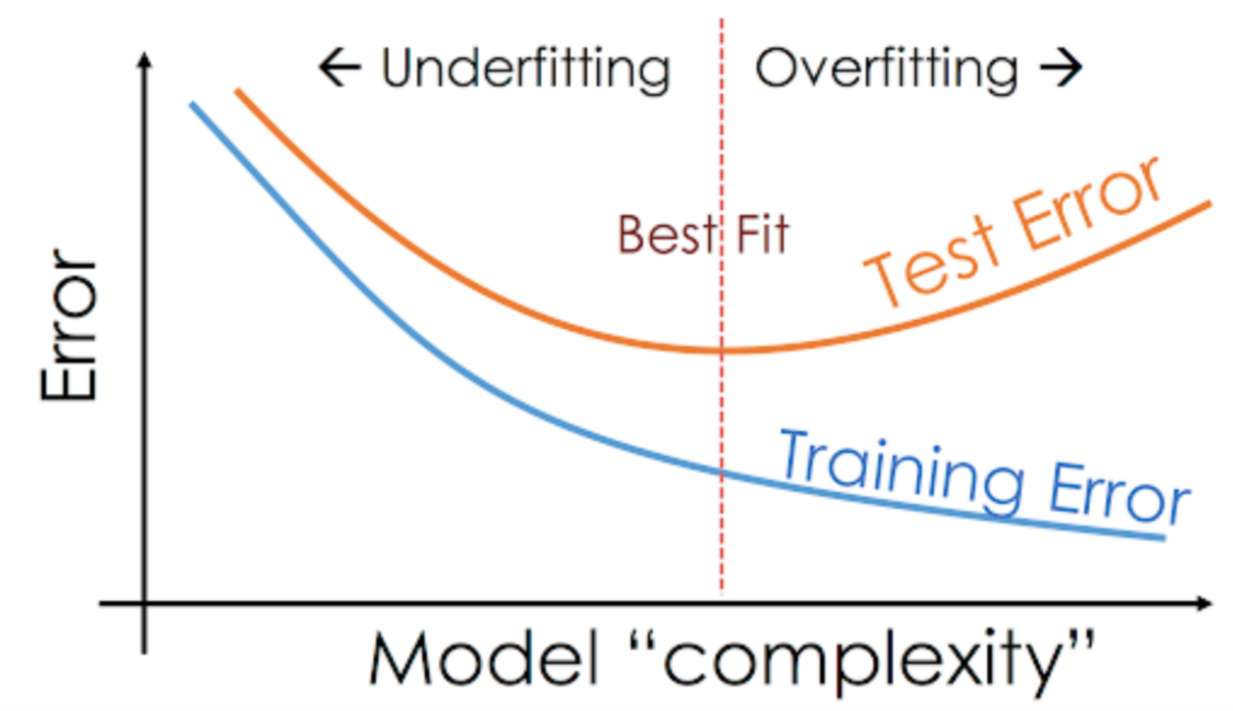
\includegraphics[width=0.5\textwidth]{./assets/modelling-ml/overfitting-vs-underfitting.jpg}
	\caption{Graph of the loss function as the number of parameters changes.}
\end{figure}

To reduce the number of parameters and ensure positive definiteness (i.e. uniqueness of the minimum)
we can use a \emph{Ridge regression} (see statistics), where we penalize the model based on the
magnitude of the parameters, this is more numerically stable.

\subsection{Bayes theorem}

\begin{equation}
	p(\theta \mid x) = \frac{p(x\mid \theta) p(\theta)}{p(x)}
\end{equation}

Our final goal is to compute the posterior $p(\theta \mid x)$.
This is hard by itself, however by using the theorem we can separate it in \say{computable}
chunks: $p(x \mid \theta)$ is the easiest; while the prior $p(\theta)$
is definitely more \say{guessable}.

Instead of minimizing the negative maximum likelihood estimator
we minimize the negative log-posterior
using a technique called \emph{maximum a posteriori} estimation.
\begin{equation}
	\argmin_\theta - \log [p(x \mid \theta) p(\theta)]
\end{equation}

\subsection{Kullback-Leibler divergence}

The definition of the KL divergence is
\begin{equation}
	D_{KL}(p,q) = \sum_{x \in X} p(x) \log \frac{p(x)}{q(x)}
\end{equation}
This is a way to measure the distance between two functions.
We can use this to minimize the distance between the given data and some theoretical distribution.
We can model the empirical data into an actual distribution by considering its histogram:
this distribution will just be a sum of $\delta$ functions of the observations we had.

\begin{proposition}{Non-negativity of DL-divergence}{dl-non-neg}
	For all probability measures $p, q$ we have that $D_{KL}(p, q) \geq 0$.
\end{proposition}

\begin{proof}
	First invert the sign of the definition:
	\begin{align}
		-D_{KL}(p,q)          & = -\sum_{x \in X} p(x) \log \frac{p(x)}{q(x)}   \\
		                      & = \sum_{x \in X} p(x) \log \frac{q(x)}{p(x)}    \\
		                      & \leq \log \sum_{x \in X} p(x) \frac{q(x)}{p(x)} \\
		                      & = \log \sum_{x \in X} q(x)                      \\
		                      & = \log (1) = 0                                  \\
		\implies D_{KL}(p, q) & \geq 0
	\end{align}
	where we have used Jensen inequality.
\end{proof}

\subsubsection{KL divergence and MLE}

We can use this distance in order to \say{fit} a model to some data:
we set $P$ to be the distribution of the empirical data, defined as
\begin{equation}
	P(x) = \frac{1}{M} \sum^M_{\mu = 1} \delta(x, x^\mu)
\end{equation}
where $\delta(x, x^\mu)$ is $1$ when $x$ is equal to the empirical sample data and $0$ otherwise.
$Q_\theta(x)$ is the approximating probability distribution.

Turns out that minimizing the KL divergence is equivalent to maximizing the MLE.

\begin{proposition}{KL divergence and MLE}{kl-mle}
	Let $P$ be the empirical distribution of the sample and $Q_\theta$ the model distribution
	parametrized by $\theta$.
	Then minimizing the KL divergence is equivalent to maximizing the MLE for $\theta$:
	\begin{equation}
		\argmin_\theta D_{KL}(P, Q_\theta) = \argmax_\theta \frac{1}{M} \sum^M_{\mu = 1} \log
		Q_\theta(x^\mu)
	\end{equation}
\end{proposition}
\begin{proof}
	We start by rewriting the KL distance:
	\begin{align}
		D_{KL}(P, Q_\theta) & = \sum_x P(x) \log \frac{P(x)}{Q_\theta(x)}                                                                                   \\
		                    & = \sum_x \frac{1}{M} \sum^M_{\mu = 1} \delta(x, x^\mu) \log \frac{\frac{1}{M} \sum^M_{\mu = 1} \delta(x, x^\mu)}{Q_\theta(x)} \\
		                    & = \frac{1}{M} \sum^M_{\mu = 1} \log \frac{\frac{1}{M}}{Q_\theta(x^\mu)}                                                       \\
		                    & = \frac{1}{M} \sum^M_{\mu = 1}\left( \log \frac{1}{M} - \log Q_\theta(x^\mu) \right)                                          \\
		                    & = -\underbrace{\log M}_\text{const} - \frac{1}{M} \sum^M_{\mu = 1} \log Q_\theta(x^\mu)
	\end{align}
	where the first term is a constant and we recognize the second term to be the MLE.
\end{proof}

\section{Dimensionality reduction}

Many times we need to analyze very high dimensional data: this is usually very hard to analyze,
almost impossible to visualize and storing it can be expensive.
We want to project our high dimensional data onto a lower dimensional space, however we want to do
this in a smart way, such that we lose the least information possible.

\subsection{The setting}

We will use a linear setting for simplicity.

Our setup is defined as a dataset $\vec X = \{ \vec x_1, \dots, \vec x_N\}$
with each $\vec x_i \in \R^D$, also assume that they are i.i.d. and with mean $0$.
Then define the \emph{data covariance matrix} as
\begin{equation}
	S = \frac{1}{M} \sum_{i = 1}^N \vec x_i \vec x_i^T
\end{equation}

We will want to project to a space of dimension $M$. If we assume $M = D$, then we can have
an invertible matrix $B$ that projects $\bm X$ onto $\R^M$ and $B^{-1}$ which does the opposite
without any error.

However, $M < B$, therefore $B$ is not a square matrix hence not invertible.
Our goal is to find a matrix $B$ such that $\vec z_i = B^T \vec x_i$ and
$\tilde{\vec x_i} = B \vec z_i$ and the error, defined as
\begin{equation}
	\norm{\vec x_i - \tilde{\vec x_i}}^2
\end{equation}
is as small as possible.
We call $B^T$ the \emph{encoder} and $B$ the \emph{decoder}.
Moreover, we want $B^T$ to be \textbf{orthonormal},
that is its columns $\vec b_i$ have $\norm{\vec b_i} = 1$ and $\vec b_i \cdot \vec b_j = 0$.

\subsection{Eigendecomposition}

In order to preserve as much data as possible we want to project in the direction that preserves
the maximum variance in the output.

We want to find vectors $b_1, \dots, b_M \in \R^D$ which will be the columns of $B^T$
Consider some vector $\vec b_i$, we want that projecting the data in its direction
$\vec z_{in} = \vec b_i^T \vec x_n \in \R$ has maximum variance:
\begin{align}
	V_i & = \mathrm{var} (\vec z_i) = \frac{1}{N} \sum^N_{j = 1} \vec z_{ij}^2               \\
	    & = \frac{1}{N} \sum^N_{j = 1} (\vec b_i^T \cdot \vec x_n)^2                         \\
	    & = \frac{1}{N} \sum^N_{j = 1} \vec b_i^T \vec x_n \vec x_n^T \vec b_i               \\
	    & = \vec b_i^T \left(\frac{1}{N} \sum^N_{j = 1} \vec x_n \vec x_n^T \right) \vec b_i \\
	    & = \vec b_i^T S \vec b_i
\end{align}
where we have used the symmetry of the product $\vec a^T \vec b = \vec a \vec b^T$.
We have obtained the so called \emph{data covariance matrix}: this is an $n \cross n$
\emph{symmetric} matrix.

\begin{theorem}{Eigendecomposition for PCA}{eigendecomposition}
	The orthonormal matrix $B^T$ which maximizes variance of the projected data
	for each input $\vec x_n$	have as its columns the eigenvectors of $S$
	with the largest eigenvalues.
\end{theorem}

\begin{proof}
	First, note that the existance of an orthonormal basis of eigenvectors of $S$ is guaranteed by
	the spectral theorem.

	We will proceed by induction, adding one by one each vector $\vec b_i$ in our basis.
		{
			\setlist{font=\normalfont\itshape}
			\begin{description}
				\item[Base case]
				      We want to solve
				      \begin{align}
					      \max_{\vec b_1} \vec b_1^T S \vec b_1 &                       \\
					      \text{subject to }                    & \norm{\vec b_1}^2 = 1
				      \end{align}

				      The lagrangian is
				      \begin{equation}
					      \mathcal L(\vec b_1, \lambda) = \vec b_1^T S \vec b_1 + \lambda(1-\vec b_1 \vec b_1^T)
				      \end{equation}
				      and setting its derivatives equal to zero we get that $S \vec b_1 = \lambda \vec b_1$
				      and $\vec b_1^T \vec b_1 = 1$.

				      By substituting we obtain
				      \begin{equation}
					      V_1 = \vec b_1^T S \vec b_1 = \lambda \vec b_1^T \vec b_1 = \lambda_1
				      \end{equation}
				      which confirms that $\vec b_1$ is an eigenvector of $S$.
				      Moreover, $V_1 = \lambda_1$ (the eigenvalue of $\vec b_1$), therefore we choose
				      $\vec b_1$ to be the eigenvectors with largest eigenvalue within the orthonormal basis
				      of $S$.

				\item[Inductive step] Assume we already have $b_1, \dots, b_k$ orthonormal eigenvectors
				      vectors of $S$ and we want to show that the next best orthonormal vector
				      $\vec b_{k+1}$ is also an eigenvector of $S$.

				      We want to solve
				      \begin{align}
					      \max_{\vec b_{k+1}}  \vec b_{k+1}^T S \vec b_{k+1} &                                                             \\
					      \text{subject to }                                 & \norm{\vec b_{k+1}}^2 = 1                                   \\
					                                                         & \vec b_{k+1}^T \vec b_i = 0 \quad \forall i \in 1, \dots, k
				      \end{align}
				      which gives us the lagrangian
				      \begin{equation}
					      \mathcal L(\vec b_1,\dots, \vec b_{k+1}, \lambda, \eta_1, \dots, \eta_k)
					      = \vec b_1^T S \vec b_1 - \lambda(\vec b_1 \vec b_1^T -1)
					      - \sum_{i = 1}^k \eta_i \vec b_{k+1}^T \vec b_i
				      \end{equation}
				      (note that we can change the signs pretty much the way we like,
				      we can incorporate the change of sign inside $\lambda$ or $\eta_i$.)

				      We take the derivative with respect to $\vec b_{k+1}$ and set it equal to zero
				      \begin{equation}
					      \pdv{\mathcal L}{\vec b_{k+1}} = 2 S \vec b_{k+1} - 2 \lambda \vec b_{k+1}
					      - \sum_{i = 1}^k \eta_i \vec b_i = 0
					      \label{eq:pca-lagrangian}
				      \end{equation}

				      Now, multiply both sides by $\vec b_j^T$ with $j \in 1, \dots, k$ so that
				      \begin{align}
					      0 & = 2 \vec b_j^T S \vec b_{k+1} - 2 \lambda \vec b_j^T \vec b_{k+1} - \sum_{i = 1}^k \eta_i \vec b_j^T \vec b_i \\
					        & = 2 \lambda_j \vec b_j^T \vec b_{k+1} - 0 - \eta_j                                                            \\
					        & = \eta_j                                                                                                      \\
				      \end{align}
				      where we have used the fact that $\vec b_j$ is an eigenvectors of $S$ and $\vec b_j$
				      is orthonormal to the other $\vec b_i$ and to $\vec b_{k+1}$.

				      We have obtained that $\eta_j = 0$ for any $j$, therefore, substituting this result
				      in \cref{eq:pca-lagrangian}, we obtain
				      \begin{equation}
					      S \vec b_{k+1} = \lambda \vec b_{k+1}
				      \end{equation}
				      which tells us that $\vec b_{k+1}$ is also an eigenvector of $S$ and gives us that
				      $V_{k+1} = \lambda$.
				      \qedhere
			\end{description}
		}
\end{proof}

\subsubsection{Data compression prospective}
It can be proven that the same conclusion would be reached if we tried to minimize the mean square
error instead.

In the end, performing some (a lot) of algebra on the mean square error we reach the same variance
formula we had before.

\subsection{Principal component analysis}

Our algorithm is then as follows:
\begin{enumerate}[label=\roman*.]
	\item Shift by the mean
	\item Scale by the variance of each dimension of the dataset
	\item Apply eigendecomposition
	\item Project along the chosen direction
\end{enumerate}

Moreover, we can prove (see slides, lecture 3), that minimizing the reconstruction error
is equivalent to finding the projected maximum variance.

\subsection{Non linear encoders}
To achieve better results we can have, on top of the linear transformation, some non-linear function,
this of course adds complexity but also gives better results.

For some $f, g$ non-linear write
\begin{align}
	\vec z          & = f(W \vec x) \\
	\vec {\tilde x} & = g(V \vec z)
\end{align}

This could lead to way better results at the price of a much larger complexity.

\section{Entropy}

\subsection{Definition}

Given a probability measure $P(x)$ we define the (Shannon) entropy as
\begin{equation}
	h(x) = \log_2 \frac{1}{P(x)}
\end{equation}
Entropy is the measure of the \say{surprise}, the more the event $x$ is unlikely, the larger the
entropy.
We can also define the average entropy of some sample $X$
\begin{equation}
	H(X) = \sum_{x \in X} P(x) \log_2 \frac{1}{P(x)} = \mathds{E}_x[h(x)]
\end{equation}

\subsubsection{Derivation}

The definition of entropy comes from four fundamental axioms about the amount of information $I(x)$
carried by each event. Consider two events $x, y$ with probabilities $p, q$:
\begin{enumerate}
	\item \emph{Normalization}: If $P(x) = 1$ then $I(p) = 0$.
	\item \emph{Monotonicity}: If $P(x) > P(y)$ then $I(p) < I(q)$.
	\item \emph{Continuity}: $I(p)$ is continuous in $p$.
	\item \emph{Additivity} for independent events: If $x \indep y$ then $I(pq) = I(p) + I(q)$.
\end{enumerate}

We can use these axioms to identify that any entropy function must have the form of
\begin{equation}
	I(p) = -C \ln p \quad \text {with } C > 0
\end{equation}
Indeed, Shannon entropy respects this result, since all logarithms are the same up to multiplication
by a constant.

\subsubsection{Information gain}

We define the conditional entropy as
\begin{equation}
	H(Y \mid X = x) = - \sum_{y \in Y} P(y \mid x) \log P(y \mid x)
\end{equation}
This allows us to define the \emph{information gain} from knowing that a certain event $x$ happened:
\begin{equation}
	\mathrm{IG}(x) = H(Y) - H(Y \mid X = x)
\end{equation}

\subsection{Decision trees}

We can use information gain to ask questions about some sample we want to classify:
assume our sample is $k$ dimensional, we split the data based on some feature $x_j > \nu$ which
maximizes information gain.

To choose the right feature $x_j$ and the right value of $\nu$ note that, even though $\nu \in \R$,
our sample is finite, therefore we only have a finite number of values $x_j$ can take which means
we only have a finite number of splits: for each $j \in 1, \dots, k$ we can just test each value
that $x_j$ takes and find the split that maximizes information gain.

Then we repeat the procedure for each split, asking a different question for each one of them, in
order to maximize the information gain each time.
We can define various criteria to stop, some of the most commons are bounding the depth of the
tree or stopping when the information gain for every choice is less than some threshold.
Note that decision trees have the tendency to overfit.

Finding the smallest consistent tree is a very complicated problem (NP-hard), however our greedy
algorithm still gives ok results.

\subsubsection{Random forests}

An even more effective way of using decision trees through the technique of
\emph{ensamble learning}, which means we take many models and the prediction is the result of a
majority vote or the average of each model.

This is useful as we can prove that averaging many i.i.d. random variables we obtain one with the
same mean but smaller variance.

Since the trees are deterministic (given the same input and hyperparameters they will produce the
same output) we differentiate them by sampling different portions of the dataset or by selecting
only certain features to split on.

Random forests are still used as a benchmark in comparison to more sophisticated approaches.

\section{Clustering}

Clustering is a class of unsupervised learning algorithms which classify the input data
$\vec x_1, \dots, \vec x_N \in X$ into $K \in \N$ partitions of $X$.
The input to the algorithm are the data $\vec x_1, \dots, \vec x_N \in X$, the number of clusters
$K$ and a distance function $d: X \cross X \to \R$.


\begin{definition}{Distance function}{distance-function}
	A function $d: X \cross X \to \R$ is a distance function on $X$ if
	\begin{enumerate}[label=\roman*.]
		\item \emph{Non-negativity}: $d(x, y) \geq 0$ for all $x, y \in X$.
		\item \emph{Identity}: $d(x, y) = 0$ if and only if $x = y$.
		\item \emph{Symmetry}: $d(x, y) = d(y, x)$ for all $x, y \in X$.
		\item \emph{Triangle inequality}: $d(x, z) \leq d(x, y) + d(y, z)$ for all $x, y, z \in X$.
	\end{enumerate}
\end{definition}

In our applications usually $X = \R^d$ and $d$ is one of the Minkowski metrics.

\begin{definition}{Minkowski metrics}{minkowski-metrics}
	Given a parameter $p \in \N$ we define the Minkowski distance on $\R^d$ as
	\begin{equation}
		d_p(\vec x, \vec y) = \left( \sum_{i = 1}^D \abs{x_i - y_i}^p\right)^{\frac{1}{p}}
	\end{equation}

	In particular:
	\begin{itemize}
		\item When $p = 1$ we obtain the \emph{Manhattan distance};
		\item When $p = 2$ we obtain the \emph{Euclidean distance};
		\item When $p \to \infty$ we obtain the \emph{Chebyshev distance}, that is
		      \begin{equation}
			      d_\infty(\vec x, \vec y) = \max_i (\abs{x_i - y_i})
		      \end{equation}
	\end{itemize}
\end{definition}

\subsection{Hierarchical algorithms}

This algorithm starts with $N$ clusters, one for each sample, and starts merging them based on the
distance between each cluster.
We could also do the opposite: start with one big cluster and split it up, but we will not focus on
this.

Starting from $N$ clusters we look for the two clusters with the smallest distance between them and
we merge them. Then we update the distance matrix between this new cluster and all the others and
repeat until we only have $K$ clusters left.

There are many ways to define the distance between two clusters $d(c_i, c_j)$:
\begin{itemize}
	\item \emph{Single linkage}:
	      \begin{equation}
		      d(c_i, c_j) = \min_{\substack{a \in c_i \\ b \in c_j}} d(a, b)
	      \end{equation}

	\item \emph{Complete linkage}:
	      \begin{equation}
		      d(c_i, c_j) = \max_{\substack{a \in c_i \\ b \in c_j}} d(a, b)
	      \end{equation}

	\item \emph{Average linkage}:
	      \begin{equation}
		      d(c_i, c_j) = \frac{1}{\abs{c_i} \abs{c_j}}
		      \sum_{\substack{a \in c_i \\ b \in c_j}} d(a, b)
	      \end{equation}
\end{itemize}

This procedure is $O(N^2)$ and it is a totally greedy approach.

The output of this algorithm is either the partition of $X$ or a \emph{dentrogram} (see
\cref{fig:dendrogram}).
These are also useful to find outliers (see lecture notes for example).

\begin{figure}[ht!]
	\centering
	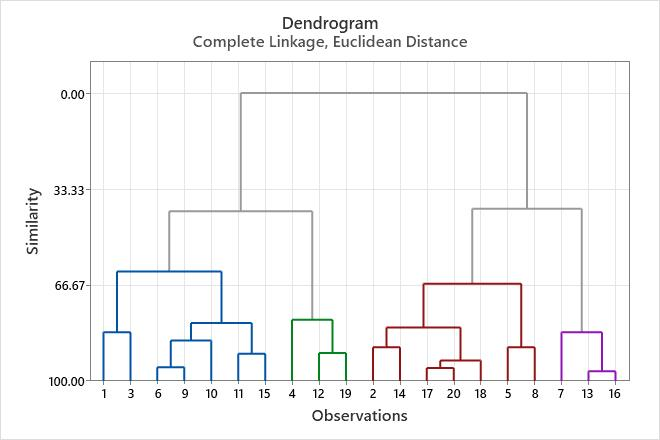
\includegraphics[width=0.5\textwidth]{./assets/modelling-ml/dendrogram.png}
	\caption{A dendrogram.}
	\label{fig:dendrogram}
\end{figure}

\subsection{\texorpdfstring{$k$}{k}-means clustering}

In this algorithm we start by randomly picking $\vec \mu_1, \dots, \vec \mu_K \in \R^d$ which will be the
\say{centers} of our clusters.
Then we repeat the following steps until convergence:
\begin{itemize}
	\item \emph{Update samples}: for each $i \in \{1, \dots, N\}$ we put $\vec x_i$ into the
	      \say{closer} cluster.
	      \begin{equation}
		      c_i = \argmax_{j \in \{1, \dots, K\}} d(\vec x_i, \vec \mu_j)
	      \end{equation}
	      where $c_i$ is the index of the cluster of $x\vec x_i$.

	\item \emph{Update centers}: for each $j \in \{1, \dots, K\}$ we update $\vec \mu_k$ to be the
	      center of the clusters.
	      \begin{equation}
		      \vec \mu_j = \frac{\sum_{i = 1}^N \delta(c_i, j) \vec x_i}{\sum_{i = 1}^N \delta(c_i, j)}
	      \end{equation}
\end{itemize}

It is possible to prove that the algorithm will converge and that each iteration will take $O(Nk)$
but it is not possible to know how many iterations it will take to converge.

\section{\texorpdfstring{$k$}{k} Nearest Neighbours}

This is a supervised learning algorithm: we are given $N$ labelled samples $(\vec x^\mu, y^\mu)$ and
we want to decide what to do with a new sample $\vec x$.

We consider $k$ samples in the training set which are the closest (according to some distance $d$)
to $\vec x$, then we take a majority vote.

This is a nice algorithm because it yields highly non-linear decision boundaries but it comes with a
computational cost: predictions take $O(kdN)$.
Furthermore, KNN is also sensitive to noise: a few noisy samples could influence the result.

\section{Perceptron}

This is a model that tries to work similarly to the actual biological neurons.
The simplest model of a neuron looks like
\begin{equation}
	y = \Theta \left(\sum_i w_i x_i - T \right)
\end{equation}
where $y \in \{0, 1\}$ is the neuron output (either it fires or it doesn't),
$\Theta$ is the Heavisde function defined as
\begin{equation}
	\Theta(x) = \begin{cases}
		1 & \text{if } x \geq 0 \\
		0 & \text{otherwise}
	\end{cases}
\end{equation}
while $w_i$ are called weights and $x_i$ are the outputs of other connected neurons.
$T$ is the fire threshold.

By changing the weight we can modify the way that neurons fire: this is a phenomenon which happens
also in biological brains.

Depending on how the neurons are connected to each other we can define \emph{feedforward}
networks, where each neuron is connected only to some \say{next} ones, and \emph{recurrent} ones,
where we can have neurons which link back to other neurons, this for example allows for short-term.

\subsection{Learning}

There are multiple way an actor can learn: we can have an unsupervised learning where the actor
is just trying to make statistical sense of the input;
we can have reinforced learning where the actor gets a reward for a correct output, this is what
happens with dopamine in biological brain;
we can have supervised learning where the actor knows what it wants to achieve and it gets feedback
on how good or bad it did, for example trying to throw a ball at a target.

\begin{figure}[H]
	\centering
	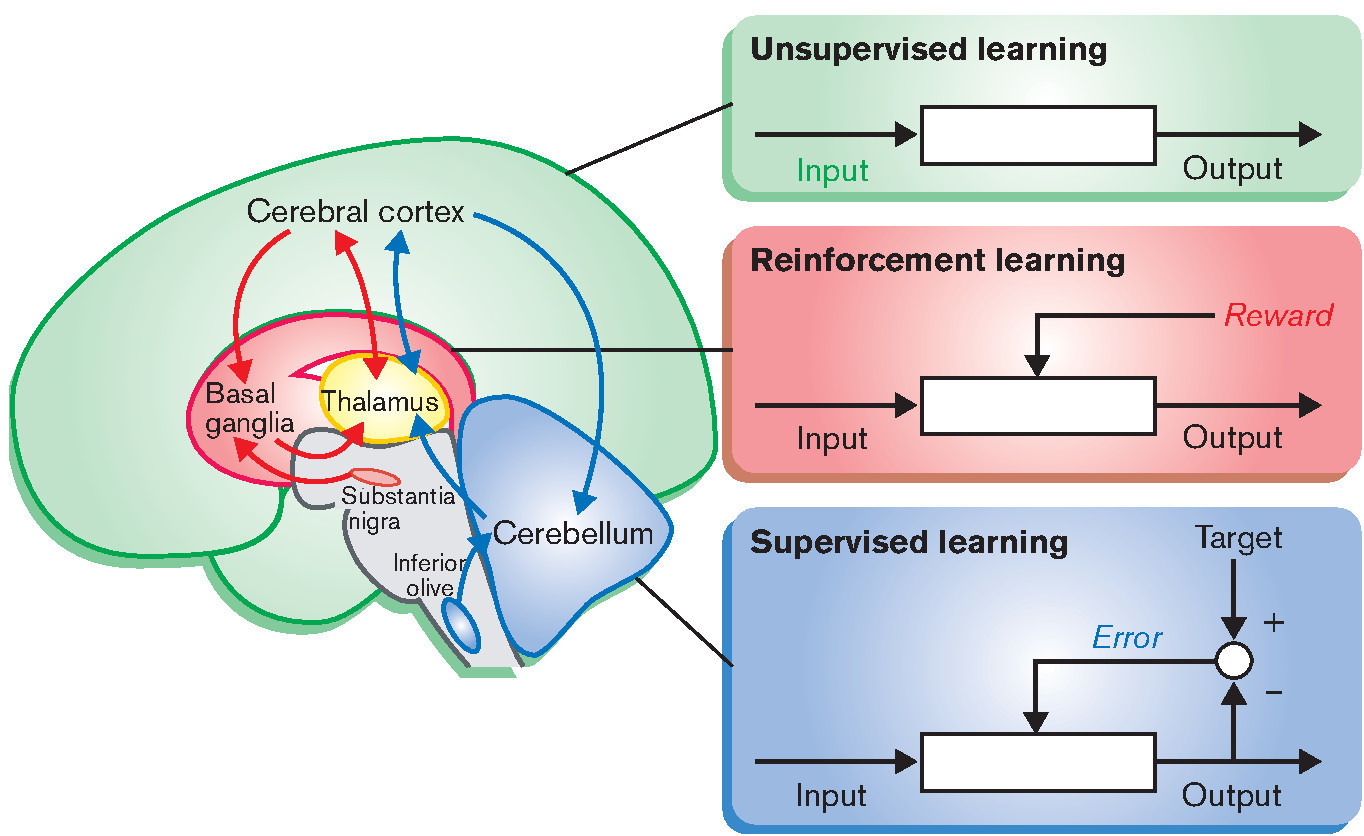
\includegraphics[width=0.5\textwidth]{./assets/modelling-ml/brain-learning-types.jpg}
	\caption{Different parts of the brain learn in different modes.}
\end{figure}

We want our model to be able to classify inputs $\vec x^\mu$ as $y^\mu \in \{0, 1\}$,
that is, we want to find some weights $\vec w$ such that
\begin{equation}
	y^\mu = \Theta(\vec w \cdot \vec x^\mu)
\end{equation}
Geometrically, this is equivalent to finding an hyperplane which divides the two sets of inputs.

A simple perceptron is able to solve problems where the inputs are already linearly separable,
for more complex inputs we will need to add hidden layers, but we will cover this further
ahead in the course.

\subsubsection{Learning algorithm}

Initialize $t = 0$ and $\vec w_t$.
Now iterate on $t$: pick a pattern $\mu$, if $\vec w_t$ gives the right output we leave it the same,
if it doesn't we modify $\vec w_{t+1}$ as follows
\begin{equation}
	\vec w_{t + 1} = \begin{cases}
		\vec w_t + \eta \vec x^\mu & \text{if } y^\mu = 1 \\
		\vec w_t - \eta \vec x^\mu & \text{if } y^\mu = 0
	\end{cases}
\end{equation}
where $\eta \in \R$ is the learning rate.

\begin{proposition}{Convergence of the perceptron algorithm}{perceptron-convergence}
	If there exists an hyperplane which separates the inputs as desired
	the perceptron algorithm will converge to it.
\end{proposition}

\begin{proof}
	We claim that if there exists $\vec w^*$ with $\norm{\vec w^*} = 1$ and
	$\vec w^* \cdot \vec z^\mu > \varepsilon$ for all $\mu$ then the algorithm will converge to it.

	For simplicity consider a learning rate $\eta = 1$
	and we let $\vec z^\mu = (2 y^\mu - 1) \vec x^\mu$ so that
	\begin{equation}
		\vec z^\mu = \begin{cases}
			\vec x^\mu  & \text{if }y^\mu = 1 \\
			-\vec x^\mu & \text{if }y^\mu = 0
		\end{cases}
	\end{equation}
	Moreover we assume that $\vec z^\mu$ is bounded, i.e. $\exists K : \norm{\vec z^\mu} < K$,
	such that $\vec w \cdot \vec z^\mu > 0$.

	The idea of this claim is that we want to find a lower bound for $A_t = \vec w_t \cdot \vec w^*$
	and an upper bound for $B_t = \norm{\vec w_t}^2$.

	Assume there exists a $\mu$ such that such $\vec w^*$ exists.
	Intialize the algorithm with $\vec w_0 = 0$ start the algorithm.
	At some time $t$ assume that $\vec w_t \cdot \vec z^\mu <0$, which means we have to perform the
	the $t+1$ modification to $\vec w$.

	For $A_{t+1}$ we have
	\begin{align}
		A_{t+1} & = (\vec w_t + \vec z^\mu) \cdot \vec w^* \\
		        & = A_t + \vec z^\mu \cdot \vec w^*        \\
		        & > A_t + \varepsilon                      \\
		        & > (t+1) \varepsilon                      \\
	\end{align}
	where in the last step we have used the fact that $A_0 = $ since $\vec w_0 = 0$ and then proceeded
	by induction.

	For $B_{t+1}$ we have
	\begin{align}
		B_{t+1} & = \norm{\vec w_t + \vec z^\mu}^2                                  \\
		        & = \norm{\vec w_t}^2 + 2 \vec w_t \vec z^\mu + \norm{\vec z^\mu}^2 \\
		        & < B_t + K^2                                                       \\
		        & < (t+1)K^2
	\end{align}
	where we have used the same induction as before and the fact that $\vec w_t \vec z^\mu < 0$.

	Now, since $A_t < \sqrt{B_t}$ for all $t$ we have
	\begin{align}
		t\varepsilon < A_t & < \sqrt{B_t} < \sqrt{t K^2} \\
		t^2 \varepsilon^2  & < t K^2                     \\
		t                  & < \frac{K^2}{\varepsilon^2}
	\end{align}
	which gives us a bound for $t$.
\end{proof}

\subsubsection{Capacity of a perceptron}
Given a set of $p$ associations $\vec x^\mu \to y^\mu$ what is the probability to find
a weight vector that correctly classifies all input patterns?

We know perceptrons can only work for patterns which are separable by an hyperplane.
Therefore our task is to find the probability that our inputs can be separated by a hyperplane.

We solve this problem geometrically, by finding the number of dichotomies of the input (that is,
what are the possible ways we can color the inputs with two colors).
In particular we look for \emph{linear dichotomies}, which are the patterns in which we can separate
the two colors with an hyperplane.

\begin{proposition}{Probability of finding a linear dichotomy}{prob-lin-dichotomy}
	The probability of finding a linear dichotomy in a set of $p$ points in $N$ dimensions is
	\begin{equation}
		P = \frac{1}{2^{p-1}} \sum_{k = 0}^{N -1} \binom{p-1}{k}
		\label{eq:prob-lin-dichotomy}
	\end{equation}
\end{proposition}

\begin{proof}
	Let $C(p, N)$ be our goal function which counts the number of linear dichotomies of $p$ points
	in $N$ dimensions.

	We know that the total number of dichotomies is $2^p$, which means that the probability of finding
	a linear dichotomy is
	\begin{equation}
		P = \frac{C(p, N)}{2^p}
	\end{equation}

	Suppose we know $C(p, N)$ and we add another point: we want to compute $C(p + 1, N)$.
	To do so we count the ways we can move the separating hyperplane without changing the output
	of the other $p$ points, but this is equivalent to counting the linear dichotomies where
	the separating hyperplane goes through a particular point.
	Since now we are constraint by passing through a point the number of dimensions
	is reduced to $N-1$, therefore we conclude that
	\begin{equation}
		C(p+1, N) = C(p, N) + C(p, N-1)
	\end{equation}

	Now we check that \cref{eq:prob-lin-dichotomy} is correct.
	Recall the way we construct Pascal's triangle: there holds that
	\begin{equation}
		\binom{p}{k} = \binom{p-1}{k} + \binom{p-1}{k-1}
	\end{equation}
	We know that $C(1, N) = 2$ and since $\binom{0}{0} = 1$ we have $C(1, N) = 2 \binom{0}{0}$.
	Then
	\begin{align}
		C(p+1, N) & = 2 \sum_{k = 1}^{N-1} \binom{p}{k}                                           \\
		          & = 2 \sum_{k = 1}^{N-1} \binom{p-1}{k} + 2 \sum_{k = 1}^{N-1} \binom{p-1}{k-1} \\
		          & = C(p, N) + 2 \sum_{k = 1}^{N-2} \binom{p-1}{k}                               \\
		          & = C(p, N) + C(p, N-1)
	\end{align}
	where we have shifted the sum by one in the third step.
\end{proof}

We can study what happens in the limit:
\begin{itemize}
	\item $p \leq N \implies P = 1$;
	\item $N \leq p \leq 2N \implies P \to 1$ as $N \to \infty$;
	\item $p = 2N \implies P = 0.5$
	\item $p > 2N \implies P \to 0$ as $N\to \infty$.
\end{itemize}
We notice that we have a very sharp bound at $p = 2N$ which separates the cases where $P = 0$ and
the ones where $P = 1$. We call $p = 2N$ the \emph{capacity} of the perceptron.

\subsubsection{Continuous perceptron}
If $y^\mu$ is a continuous variable, instead of being in $\{0, 1\}$, we need to define a cost
function $\phi$ such that

TODO

\section{Auto encoder}

\subsection{Gradient descent}
\label{sec:gradient-descent}
\subsubsection{Loss function}

To do supervised learning ideally we'd like to minimize the error rate on the training set.
\begin{equation}
	\min_{\vec w} \frac{1}{N} \sum_{i = 1}^N \mathds 1(y_i \neq y(\vec w, \vec x))
\end{equation}
but this is very hard (NP-hard, in fact). We want to take a relaxation of this.

Consider
\begin{equation}
	\min_{\vec w} \frac{1}{N} \sum_{i = 1}^N \ell(y_i, \vec w, \vec x)
\end{equation}
for some \emph{surrogate loss function} $\ell$.

How do we choose the right $\ell$? We want it to be differentiable, sensitive to changes in
$\vec w$, but not necessarily convex.
Convexity would be nice because then we are guaranteed to have an unique minimum but in reality we
often do not have this pleasure.

Some example of surrogate loss functions are the square loss function or the logistic loss function.

\subsubsection{Idea of gradient descent}

We want to update the weight $\vec w$ so that the loss function decreases.

\begin{equation}
	\vec w_{t} = \vec w_{t-1} - \eta_t \grad \left(\frac{1}{N}\sum_{i = 1}^N
	\ell(\vec w_{t-1}, \vec x_i, y_i) \right)
\end{equation}
where $\eta_1, \dots, \eta_K$ is the learning rate. We take it as a sequence since we might want to
change it: at the beginning we want to take bigger steps, then we take smaller ones in order to
fine-tune the result.

For the square loss function $\ell(\vec w, \vec x, y) = (y_i - \vec w \cdot \vec x_i)^2$
\begin{align}
	\vec w_{t} & = \vec w_{t-1} - \eta_t \grad \left(\frac{1}{N}\sum_{i = 1}^N (y_i - \vec w \cdot \vec x_i)^2 \right) \\
	           & = \vec w_{t-1} - \eta_t  \frac{1}{N}\sum_{i = 1}^N 2 (y_i - \vec w \cdot \vec x_i) \vec x_i           \\
	           & = \vec w_{t-1} - \eta_t  \frac{1}{N}\sum_{i = 1}^N (y_i - \vec w \cdot \vec x_i) \vec x_i
\end{align}
where we have absorbed the $2$ into $\eta_t$.

The costly part of our algorithm is the sum we over $N$: at every iteration the need to sum over all
the dataset is very expensive.

\subsubsection{Mini-batch}
\label{sec:mini-batch}

Instead of averaging over the whole dataset, at each iteration $t$ we choose a set $B_t$ with
$\abs{B_t} = m$ uniformly at random within the data set.

\begin{equation}
	\vec w_{t} = \vec w_{t-1} - \eta_t  \frac{1}{m}\sum_{(\vec x, y) \in B_t}
	(y_i - \vec w \cdot \vec x_i) \vec x_i
\end{equation}

Note that a higher $m$ gives lower variance but it is also more computational expensive.

This algorithm makes use of a lot of linear algebra, which is easily parallelizable on GPUs.

Moreover, we can use a regularization term (as in ridge regression) to avoid $\vec w$ from getting
too big.
\begin{equation}
	\min_{\vec w} \frac{1}{N} \sum_{i = 1}^N (y_i - \vec w \cdot \vec x) + \lambda \norm{\vec w}^2
\end{equation}

\subsection{MLP autoencoders}

A multi-layer perceptron is a device similar to a perceptron: the inputs are multiplied by some
weights and trigger the activation of a node. However, differently from the perceptron case, each
layer has more than one node: the weighted inputs are passed to multiple perceptrons with different
weights. In turn, the output of these perceptrons will be weighted again and passed over as the
input for the next layer.
Moreover, the nodes will have some (maybe different) activation function.

We have a lot of weights! Each layer has its own.
\begin{equation}
	W_{ij}^{(k)} \quad \text{where } \begin{cases}
		i \text{ is the index of the starting node/input}     \\
		j \text{ is the index of the destination note/output} \\
		k \text{ is the index of the layer}
	\end{cases}
\end{equation}

We can divide this network in three parts: an encode, a decoder and a feature generating layer.
The \textbf{encoder} is the first part of the network, which takes the input data and creates a
\emph{latent feature representation} of it.
The \textbf{decoder} takes the output of the network and reconstruct a result which has the same
shape as the original input.

Given an input $\vec x_i \in \R^d$, the encoder will construct an internal representation
$\vec z_i \in \R^q$ with $d > q$: this encoding process can be \say{summarized} by a function
$g_{\vec w}: \R^d \to \R^q$ (which is the composition of linear and non-linear functions).
Then the decoder takes the encoded data and decodes it, therefore the reconstructed data is
$\tilde{\vec x}_i = f_{\vec w'}(g_{\vec w}(\vec x_i))$ where $f_{\vec w'}$ is the work done by the
decoder.

To train this network we want to find some $\vec w, \vec w'$ such that
\begin{equation}
	(\vec w, \vec w') = \argmin_{ \vec w, \vec w' }
	\E [ \ell( \vec x_i, f_{\vec w'}(g_{\vec w}(x_i))]
\end{equation}
where $\E$ is just a fancy way to say average.

To this we can add some $L^1$ or $L^2$ normalization terms and then run gradient descent on this.
We have obtained a non-linear compressor, yay!

\subsubsection{Activation functions}

As we said, the non linearity comes from the activation functions of each neuron.
There are many choices of these functions but the most popular are
\begin{itemize}
	\item \emph{ReLU}: this function is good for when the input takes a wide range of positive real
	      values.
	      \begin{equation}
		      \mathrm{ReLU}(x) = \max \{ 0, x \}
	      \end{equation}

	\item \emph{Sigmoid function}: this is good when the input $x \in (0, 1)$.
	      \begin{equation}
		      \sigma(x) = \frac{1}{1+e^{-x}}
	      \end{equation}

\end{itemize}

\subsection{Variational Autoencoders}

This methods takes a sample $\vec x$, compresses it using a traditional MLP autoencoder, and
interprets the encoded values as the parameters to a normal distribution.
This means that the output of the encoder is a mean $\mu(\vec x)$ and a standard deviation
$\sigma(\vec x)$.

Then the decoder samples a $\vec z$ from a distribution which looks like
\begin{equation}
	\vec z \sim q_\gamma(\vec z \mid \vec x) = \mathrm N (\mu(\vec x), \sigma^2(\vec x) \mathds 1)
\end{equation}
Then it decodes it back to a vector of the same dimension of $\vec x$.

This is particularly interesting as this kind of model can generate new kind of outputs similar to
the inputs it has already received.

\subsubsection{ELBO}

We'd like to maximize the MLE but this is computationally too expensive.
Instead we introduce a lower bound called ELBO.

We derive it from the MLE by introducing an approximate distribution $q(\vec z \mid \vec x)$.
\begin{align}
	\log p(\vec x) & = \E_{q(\vec z \mid \vec x)}[\log p(\vec x)]                                                             \\
	               & = \E_{q(\vec z \mid \vec x)}\left[ \log p(\vec x) - \log \frac{p(\vec x, \vec z)}{q(\vec z \mid \vec x)}
	+ \log \frac{p(\vec x, \vec z)}{q(\vec z \mid \vec x)}\right]                                                             \\
	               & = \E_{q(\vec z \mid \vec x)}\left[ \log \frac{p(\vec x)q(\vec z \mid \vec x)}{p(\vec x, \vec z)} \right]
	+ \E_{q(\vec z \mid \vec x)}\left[\log \frac{p(\vec x, \vec z)}{q(\vec z \mid \vec x)}\right]                             \\
	               & = \underbrace{\E_{q(\vec z \mid \vec x)}\left[ \log {p(\vec x \mid \vec z)} \right]}_{D_{KL}}
	+ \underbrace{\E_{q(\vec z \mid \vec x)}\left[\log \frac{p(\vec x, \vec z)}{q(\vec z \mid \vec x)}\right]}_{\mathrm{ELBO}}
\end{align}
where we have obtained that the log likelihood is just the KL divergence
$D_{KL}(q(\vec z \mid \vec x) \parallel p(\vec x \mid \vec x))$ plus this other term we will call
ELBO:
\begin{align}
	\mathrm{ELBO}(\vec x; \theta, \gamma) & =
	\E_{q_\gamma(\vec z \mid \vec x)}\left[\log \frac{p_\theta(\vec x, \vec z)}{q_\gamma(\vec z \mid \vec x)}\right] \\
	                                      & =
	\int q_\gamma(\vec z \mid \vec x) \log \frac{p_\theta(\vec x, \vec z)}{q_\gamma(\vec z \mid \vec x)} \dd \vec z
\end{align}
with $\gamma \in \Gamma$ and $\theta \in \Theta$ which are the parameters for the distributions $q$
and $p$.

Note that since $D_{KL} \geq 0$ always, we get
$\log p(x) \geq \mathrm{ELBO}(\vec x; \theta, \gamma)$.

\subsubsection{Optimization}

Now we would proceed to run gradient descent on ELBO, updating first $\gamma$ and then $\theta$,
but this is quite tricky because stochastic sampling complicates the process.
Instead we use a reparametrization trick to remove the stochasticity from the backpropagation step.

Consider $q_\gamma(\vec z \mid \vec x)$:
\begin{equation}
	q_\gamma(\vec z \mid \vec x) = \mathrm N(g(\vec x), h(\vec x)^2)
\end{equation}
for some mean $g$ and some standard deviation $h$.

To get a $z$, instead of sampling from this distribution, we sample
$\varepsilon \sim \mathrm{N}(0, \mathds 1)$ and define $z$ as
\begin{equation}
	\vec z = g(\vec x) + \varepsilon h(\vec x)
\end{equation}
where $\varepsilon$ represents the noise, which is sampled beforehand and therefore does not effect
the computation of the gradient.
In fact we get
\begin{equation}
	\pdv{\vec z}{\mu} = 1, \qquad \pdv{\vec z}{\sigma} = \varepsilon
\end{equation}

\section{Deep networks}

\subsection{Limitations of perceptrons}
As we saw, the perceptron has a lot of limitations, as we are only able to classify inputs which are
linearly separable.
We could solve this problem by adding more dimensions but this is kind of cumbersome and doesn't
always work.

Take for instance the problem of classifying some vectors $\vec x^\mu \in \{0, 1\}^n$.
We want to put each vector into a basket: basket $A$ if there exists some $j$ so that
\begin{equation}
	x^\mu_j = x^\mu_{j+1} = 1
\end{equation}
and in the basket $B$ otherwise.

Assume there exists a perceptron capable of correctly classifying any of these patterns. Since the
perceptron is linear any linear combination of any two input patterns will be classified in the same
way. But this will inevitably lead to some errors in this case, therefore we have a contradiction
and no perceptron is able to perfectly solve this problem.

\subsection{Multilayer non-linear networks}

To fix this problem we introduce non-linearity and multiple perceptron.

We will have a number $L$ of layers and for each layer will have $N_\ell$,
for $\ell \in \{1, \dots, L\}$, number of non-linear perceptrons.
Each perceptron in a certain layer is connected to every perceptron in the next one, except for
perceptrons in $\ell = 0$ which don't have any incoming connections (they are the input of the
network), and for $\ell = L$ which doesn't have any outgoing connections (they are the output of the
network).

Each perceptron has its weight vector $\vec w^\ell_i$, each component $w^\ell_{ij}$ is the weight of
the connection from perceptron $i$ in layer $\ell -1$ to perceptron $j$ in layer $\ell$.
Sometimes we consider also a bias $b^\ell_{ij}$ for each neuron which gets added on at the end, this
is the same as having an additional neuron in the previous layer which always output $1$.

Upon receiving some input $\vec x$ from the previous layer, each perceptron calculates the
preactivation value $a = \vec w \cdot \vec x + b$. Then the preactivation value is passed through a
non-linear function $f$ (which is usually the same for all neurons, except maybe for the output
layer) and then the result $f(a)$ is passed to the next layer.

This function $f$ (or some times referred as $\sigma$) is called activation function and there
are different choices of it:
\begin{itemize}
	\item \emph{ReLU (Rectified Linear Unit)}
	      \begin{equation}
		      f(x) = \max \{0, x \}
	      \end{equation}
	\item \emph{Soft ReLU}
	      \begin{equation}
		      f(x) = \ln(1 + e^x)
	      \end{equation}
	\item \emph{Hard Threshold}
	      \begin{equation}
		      f(x) =
		      \begin{cases}
			      1, & \text{if } x > 0 \\
			      0, & \text{otherwise}
		      \end{cases}
	      \end{equation}
	\item \emph{Logistic (Sigmoid)}
	      \begin{equation}
		      f(x) = \frac{1}{1 + e^{-x}}
	      \end{equation}
	\item \emph{Tanh (Hyperbolic Tangent)}
	      \begin{equation}
		      f(x) = \tanh(x) = \frac{e^x - e^{-x}}{e^x + e^{-x}}
	      \end{equation}
\end{itemize}

\begin{figure}
	\centering
	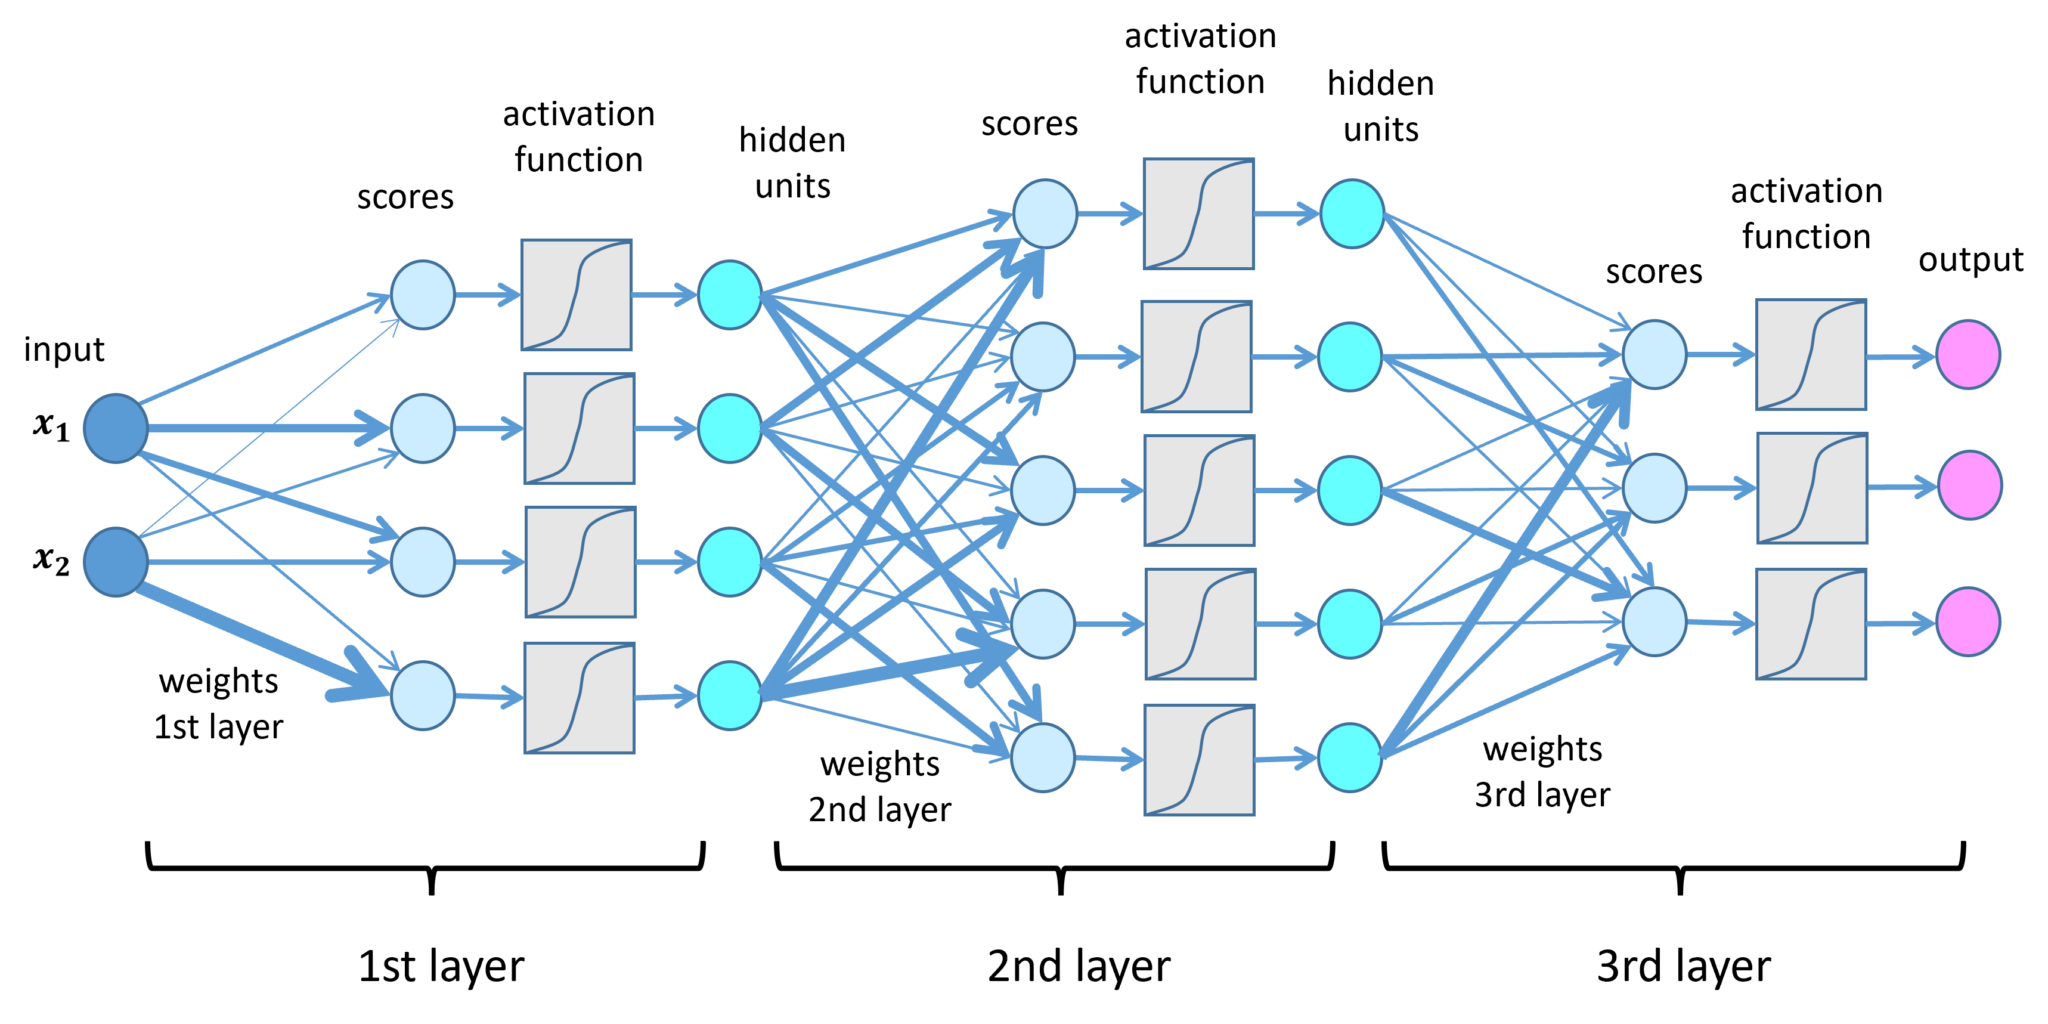
\includegraphics[width=0.9\textwidth]{./assets/modelling-ml/deep-network.png}
	\caption{Scheme of a deep network.}
\end{figure}

\begin{theorem}{Hornik}{hornik}
	Let $\sigma: \R \to \R$ be a nonconstant, bounded, non-decreasing, and continuous function.
	Let $S \subseteq \R^d$ be closed and bounded.
	Then, for any $f: S \to \R$ continuous and any $\varepsilon > 0$, there exists a neural network
	with one hidden layer containing finitely many nodes which we can write as
	\begin{equation}
		h(\vec x) = \sum_{j = 1}^k w^\text{out}_j \sigma(\vec w_j^T \vec x + b_j)
	\end{equation}
	so that, $\forall x \in S$, we have
	\begin{equation}
		\abs{f(\vec x) - h(\vec x)} < \varepsilon
	\end{equation}
\end{theorem}

This is a key theorem which tells us that any function can be learned by a neural network, however,
in practice, this has little to no utility: it doesn't tell us anything about the performance of
some specific network and doesn't tell us how to compute the weights; moreover the network of the
theorem has just one hidden layer, when in practice we have evidence that multiple hidden layers
provide significantly better results.

\subsection{Backpropagation}

The key concept behind backpropagation is gradient descent, as we covered in
\cref{sec:gradient-descent}, in practice we need to apply many times the chain rule.

Recall that at layer $\ell$, the preactivation value, given by the output $\vec z^{(\ell - 1)}$ of
layer $\ell - 1$, is defined as
\begin{equation}
	a^{(\ell)}_j = \left( \sum_{i = 1}^{d^{(\ell - 1)}} w_{ji}^{(\ell)} z_i^{(\ell - 1)}\right) +
	b_j^{(\ell)}
\end{equation}
for ease of notation we will omit the bias term since the procedure remains the same.

The output of each neuron is $z_j^{(\ell)} = \sigma(a_j^{(\ell)})$, while the output of the network
is the preactivation value of layer $L + 1$: $\hat{y} = a^{(L+1)}$.
(Note that the output is a single node).

Our loss function $L$ is defined as
\begin{equation}
	L(\vec w^{(1)}, \dots \vec w^{(L+1)}) = \frac{1}{N} \sum_{n = 1}^N \ell(y_n, \hat y_n)
	= \frac{1}{2N} \sum_{n = 1}^N (y_n - \hat y_n)^2
\end{equation}
where we used the square loss function.

Our goal is then to compute $\grad \ell (y_n, \hat y_n)$ with respect to all parameters, this
means we want to compute
\begin{equation}
	\pdv{\ell(y_n, \hat y_n)}{w_{ji}^{(\ell)}} =
	\underbrace{\pdv{\ell(y_n, \hat y_n)}{a_{j}^{(\ell)}}}_{\delta^{(\ell)}_j}
	\pdv{a_{j}^{(\ell)}}{w_{ji}^{(\ell)}}
\end{equation}
where we used the chain rule to separate the derivative. We call the first term $\delta^{(\ell)}_j$
and claim that the second term is equal to $z_i^{(\ell - 1)}$. This is due to the fact that
\begin{equation}
	a^{(\ell)}_j = \vec w_j \cdot \vec z^{(\ell -1)} = \sum_c w_{jc}^{(\ell)} z_c^{(\ell - 1)}
\end{equation}
from which we notice that taking the derivative w.r.t. $w^{(\ell)}_{ji}$ makes all the terms of the
sum go to zero except for $z_i^{(\ell - 1)}$.

We are now left with
\begin{equation}
	\pdv{\ell(y_n, \hat y_n)}{w_{ji}^{(\ell)}} = \delta^{(\ell)}_j z_i^{(\ell - 1)}
\end{equation}
Lets now work on $\vec \delta^{(\ell)}$.

At $L + 1$ we have a single node, therefore we can write
\begin{equation}
	\delta^{(L + 1)} = \pdv{\ell(y, \hat y)}{a^{(L+1)}} =  -(y- \hat y) = -\left(y - a^{(L+1)}\right)
\end{equation}
then
\begin{equation}
	\pdv{\ell(y_n, \hat y_n)}{w_{j}^{(L+1)}} =-\left(y - a^{(L+1)}\right) z_j^{(L+1)}
\end{equation}

We now want to proceed recursively: we will compute $\vec \delta^{(\ell)}$ by knowing
$\vec \delta^{(\ell + 1)}$.
\begin{equation}
	\delta^{(\ell)} = \pdv{\ell(y, \hat y)}{a_j^{(\ell)}}
	= \sum_{k = 1}^{d^{(\ell + 1)}} \pdv{\ell(y, \hat y)}{a_k^{(\ell+1)}}\pdv{a_k^{(\ell + 1)}}{a_j^{\ell}}
	= \sum_{k = 1}^{d^{(\ell + 1)}} \delta^{(\ell + 1)}_k \pdv{a_k^{(\ell + 1)}}{a_j^{\ell}}
\end{equation}

Now we are left with computing $\pdv{a_k^{(\ell + 1)}}{a_j^{\ell}}$. Since, by definition,
$a_k^{(\ell + 1)}$ is
\begin{equation}
	a_k^{(\ell + 1)} = \sum^{d^{(\ell + 1)}}_{c = 1} w_{kc}^{(\ell + 1)} z_c^{\ell}
	= \sum^{d^{(\ell + 1)}}_{c = 1} w_{kc}^{(\ell + 1)} \sigma(a_c^{\ell})
\end{equation}
giving us that
\begin{equation}
	\pdv{a_k^{(\ell + 1)}}{a_j^{\ell}} = w_{kj}^{(\ell + 1)} \sigma(a_j^{\ell})
\end{equation}
and substituting into $\vec \delta$ we obtain
\begin{equation}
	\delta^{(\ell)}_j = \sigma(a_j^{\ell}) \sum_{k = 1}^{d^{(\ell + 1)}}
	\delta_k^{(\ell + 1)} w_{kj}^{(\ell + 1)}
\end{equation}

Now that we have an formula which works we can apply gradient descent: we start by doing a
\emph{forward pass}, which means we run the network with some arbitrary weights, so that we get a
value for $\vec a^{(\ell)}$; then we compute the gradient as shown starting from the last layer
(hence the name backpropagation) and perform gradient descent to update the weights.

\subsection{Soft-max}

Assume now no longer have a binary classification problem but we want to distinguish between $K$
classes.

We train a network with $K$ output neurons $z_k$, then, we apply the soft-max function to each of
them, giving us the probability that the sample belongs to a certain class:
\begin{equation}
	P(y = \ell \mid \vec x) = a_\ell = \frac {e^{z_\ell}}{\sum_{k = 1}^{K} e^{z_k}}
\end{equation}

Note that the likelihood for a one-hot encoded target vector $\vec y$ is
\begin{equation}
	\prod_{k = 1}^K a^{y_k}_k = a_\ell
\end{equation}
where $\ell$ is the true class.

We can also define the \emph{cross entropy loss}
\begin{equation}
	L = - \sum_{k = 1}^{K} y_k \log (a_k)
\end{equation}
note that when $a_k$ correctly classifies every input the loss is exactly zero.

We now want to integrate this into the backpropagation algorithm. To do so we will need to compute
$\pdv{L}{w_kj}$, however we start by looking at $\pdv{L}{z_k}$.

\begin{align}
	\pdv{L}{z_k} & = \sum_{i = 1}^{K} \pdv{L}{a_i} \pdv{a_i}{z_k}                                                \\
	             & = \sum_{i = 1}^{K} \left( - \frac{y_i}{a_i} \right) \left( a_i (\delta_{i = k} - a_k) \right) \\
	             & = - \sum_{i = 1}^{K} y_i (\delta_{i = k} - a_k)                                               \\
	             & = - y_k + a_k \sum_{i = 1}^{K} y_i                                                            \\
	             & = a_k - y_k
\end{align}
where $\delta_{i = k}$ is the delta function and the last simplification is due to the fact that
$\vec y$ is one-hot encoded.

\section{Hopfield model}

We now tackle to problem of \say{memorizing} certain patterns so that similar patterns will be able
be recognized by our network.

Consider a network of $N$ binary neurons so that $S_i = \pm 1$ is the activation of the neuron $i$.
A pattern is a vector $\vec \xi \in \{\pm 1\}^N$ so that $\vec \xi_i = S_i$ is the desired
activation of $S_i$ for that pattern. We will have $p$ patterns we want to memorize, let us denote
them as $\vec \xi^\mu$ with $\mu \in \{1, \dots, p\}$.
Assume no correlation between the patterns.

To retrieve a memory from the network we initialize the network with some pattern and we let it run.
If it converges to some $\vec \xi^\mu$ we have successfully recognized the new pattern as
$\vec \xi^\mu$. Formally we want
\begin{equation}
	m_\mu(t) = \frac{1}{N} \sum_{i = 1}^N S_i \xi^\mu_i \xrightarrow{ N \to \infty } 1
\end{equation}
i.e. the average overlap should stay around $1$ as we increase the number of neurons, this tells us
that the new pattern is recognized as $\vec \xi^\mu$.
On the other hand, if the new pattern is uncorrelated from $\vec \xi^\mu$ we can apply the central
limit theorem to obtain that $m_\mu(t) \sim \mathrm{N}(0, N^{-1})$ and $m_\mu(t)$ converges to $0$.
The variance of $m_\mu(t)$ is calculated as
\begin{equation}
	\var (m_\mu(t)) = \frac{1}{N^2} \sum_i^N \var(S_i(t)) = \frac{1}{N}
\end{equation}



What is the best way of connecting our neurons? We will use the result hypothesised by Hebb which
tells us that we should weight the connection as the average of the patterns involved in the
connection:
\begin{equation}
	J_{ij} = \frac{1}{N} \sum_{\mu = 1}^p \xi_i^\mu \xi_j^\mu
\end{equation}

With this weights we notice that the input patterns $\vec \xi^\mu$ are fixed points of the network
when $N \gg p$.
Let us consider the pattern $\nu$.
At $t = 0$ we initialize the network to so that $S_i(t=0) = \xi^\nu_i$ for all $i$.
At the next step we will have
\begin{align}
	S_i(t=1) & = \mathrm{sign}\left( \sum_{j \neq i} J_{ij} S_j \right)                                                                                                        \\
	         & = \mathrm{sign}\left( \sum_{j \neq i} J_{ij} \xi^\nu_j \right)                                                                                                  \\
	         & = \mathrm{sign}\left( \sum_{j \neq i} \left(\frac{1}{N} \sum_{\mu = 1}^p \xi_i^\mu \xi_j^\mu\right) \xi^\nu_j \right)                                           \\
	         & = \mathrm{sign}\left( \frac{1}{N} \sum_{j \neq i} \xi^\nu_i \cancelto{1}{(\xi^\nu_j)^2} + \frac{1}{N} \sum_{\mu \neq \nu} \xi_i^\mu \xi_j^\mu \xi^\nu_j \right) \\
	         & = \mathrm{sign}\left( \xi^\nu_i + \frac{1}{N} \sum_{j \neq i} \sum_{\mu \neq \nu} \xi_i^\mu \xi_j^\mu \xi^\nu_j \right)
\end{align}
where we notice that the second (noise) term goes to $0$ as $N \gg p$.

However, how much bigger does $N$ has to be?
Assume $p = \alpha N$, then we can show using probability sorcery to show that the minimum $\alpha$
such that equilibrium points still exist is $\alpha_c = 0.14$.

\section{Boltzmann machines}
This is a type of network to do unsupervised learning: given a set of examples it tries to recover
the original distribution and can be then used to generate new samples from the same distribution.

A Boltzmann machine is made of $N$ binary neurons $S_i(t) \in \{0, 1\}$ with symmetric connectivity.
The neurons in this network can be divided in two layer: an input layer and a hidden one.
If the neurons are connected in such way that the input and hidden layer form two parties of a
bipartite graph we have a \emph{restricted Boltzmann machine} (RBM).
We will focus on RBMs as the learning algorithm is much simpler and faster.

We will call $\vec w$ the 2D matrix of weights, while $\vec h$ value taken by the hidden neurons,
$\vec v$ are the values taken by the visible layer. Finally $\vec b$ is the bias of the hidden
neurons and $\vec c$ is the bias of the visible neurons.

\subsection{Updating}

In an RBM each neuron is updated as follows:
\begin{itemize}
	\item Compute the weighted sum of its inputs:
	      \begin{equation}
		      z_i = b_i + \sum_j w_{ij} S_j
	      \end{equation}
	      where $b_i$ is the bias.
	\item The state of each neuron is not deterministic, instead the probability of the neuron
	      firing is given by
	      \begin{equation}
		      P(S_i = 1) = \frac{1}{1 + e^{-z}}
	      \end{equation}

	\item Eventually the network reaches a stationary distribution called
	      \emph{Boltzmann distribution} given by
	      \begin{equation}
		      P(S) = \frac{1}{Z} \exp (-E(S))
	      \end{equation}
	      where
	      \begin{align}
		      Z    & = \sum_{S} E(S)                                  \\
		      E(S) & = - \sum_{i < j} w_{ij} S_i S_j - \sum_i b_i S_i
	      \end{align}
	      where $Z$ is the sum of the energy of all states and $E(S)$ is the energy of the state $S$,
	      which is given by the weighted sum of the activation of the neurons (the first term
	      represents the connection between the two layers and the second one the bias of each
	      neuron).

	\item Then we proceed by updating the hidden units:
	      \begin{equation}
		      P(\vec h_j = 1) = \sigma \left( \sum_k \vec w_{jk} \vec x_k + \vec b_j \right)
	      \end{equation}
	      and then the visible units
	      \begin{equation}
		      P(\vec x_k = 1) = \sigma \left( \sum_j \vec w_{kj} \vec h_j + \vec c_j \right)
	      \end{equation}
	      where $\sigma$ is the sigmoid function
	      \begin{equation}
		      \sigma(x) = \frac{1}{1 + e^{-x}}
	      \end{equation}

\end{itemize}

\subsection{Training}

We train this network with the goal to maximize the log-likelihood of the data, i.e.
\begin{equation}
	C = \frac{1}{M} \sum_{\mu = 1}^M \log P(x^\mu)
\end{equation}

\subsubsection{Gradient descent}

Of course we can use GD, therefore we need to compute the derivatives
w.r.t. the parameters $\theta = (\vec w, \vec b)$.
\begin{equation}
	\pdv{C}{\theta} = \frac{1}{M} \sum^M_{\mu = 1}
	\E\left[ \pdv{E(\vec x^\mu, \vec h)}{\theta} \right] - \E\left[ \pdv{E(\vec x, \vec h)}{\theta} \right]
	\label{eq:rbm-gd}
\end{equation}
where we are taking the mean over $S$ using the Boltzmann distribution.

Then we update the parameters as follows
\begin{align}
	\Delta \vec w_{jk} & = \eta
	\left( \frac{1}{M} \sum_{\mu}^{} \E_h[\vec h_j \vec x_k^\mu] - \E_{x, h}[\vec h_j \vec x_k] \right) \\
	\Delta \vec b_{j}  & = \eta
	\left( \frac{1}{M} \sum_{\mu}^{} \E_h[\vec h_j] - \E_{h}[\vec h_j] \right)                          \\
	\Delta \vec c_{k}  & = \eta
	\left( \frac{1}{M} \sum_{\mu}^{} \vec x_k - \E_{x}[\vec x_k] \right)
\end{align}
where $\eta$ is the learning rate.

However computing the average over all possible values of $\vec x$ and $\vec h$ is impractical.
We often choose a mini-batch approach instead or a different technique all together.

\subsubsection{Contrastive divergence}

To avoid the computational cost we replace the negative term in \cref{eq:rbm-gd} with a single point
estimate $\tilde {\vec x}, \tilde {\vec h}$.

We perform $k$ steps of Gibbs sampling: we start with a training example $\vec x^{(0)}$, then we
sample a hidden state $\vec{h}^{(0)}$ from \(P(\vec{h}|\vec{v}^{(0)})\). We then proceed by
reconstructing a visible state \(\vec{x}^{(1)}\) from \(\vec{h}^{(0)}\) by sampling from
\(P(\vec{v}|\vec{h}^{(0)})\), then we sample a new hidden state \(\vec{h}^{(1)}\) from it and so on,
until we reach $k$.

\subsection{In practice}

We need to choose the right number of nodes per layer, learning rate, initial values, batch sizes,
etc.

Moreover we often stack more RBMs: we train them one layer at the time and then the hidden neurons
of one layer become the inputs to the next one.


\end{document}
